% --
% machine learning

\section{Neural Networks for KWS}
\sectionheader{Neural Networks for KWS}

\begin{frame}
  \frametitle{Fully Connected Layer}
  \vspace{-0.75cm}
  \begin{columns}
    \begin{column}{0.5\textwidth}
      \begin{itemize}
        \small
        \item Math. formulation:
        \begin{equation*}
          \footnotesize
          \bm{z} = h(W \bm{x} + \bm{b})
        \end{equation*}
        \footnotesize
        with $\bm{x} \in \R^n$, $\bm{z} \in \R^m$, $\bm{b} \in \R^m$.
        \small
        \vspace{0.2cm}
        \item Amount of Params: 
        \footnotesize 
        $m \cdot n + m$
        \small
        \vspace{0.2cm}
        \item Amount of Operatios:
        \begin{equation*}
          \footnotesize
          \mathcal{T}(W \bm{x} + \bm{b}) \approx 2 (m \cdot n) + m
        \end{equation*}     
      \end{itemize}
    \end{column}
    \begin{column}{0.5\textwidth}
      \vspace{0.75cm}
      \centering
      \begin{figure} 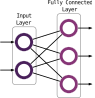
\includegraphics[width=0.6\textwidth]{../4_nn/figs/nn_theory_fc.pdf} \end{figure}
      \vfill
    \end{column}
  \end{columns}
\end{frame}

\begin{frame}
  \frametitle{Convolutional Neural Networks}
  \begin{figure} 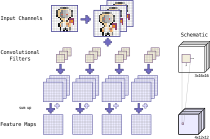
\includegraphics[width=0.8\textwidth]{../4_nn/figs/nn_theory_cnn_basics.pdf} \end{figure}
\end{frame}

\begin{frame}
  \frametitle{Traditional Network (conv-trad)}
  \vspace{-0.5cm}
  \begin{itemize}
    \small
    \item Layer Structure: Conv.: 2 + 1 max. pol, FC: 3 
    \item Num. Params:
    \item Num. Operations: 
  \end{itemize}
  \begin{figure} 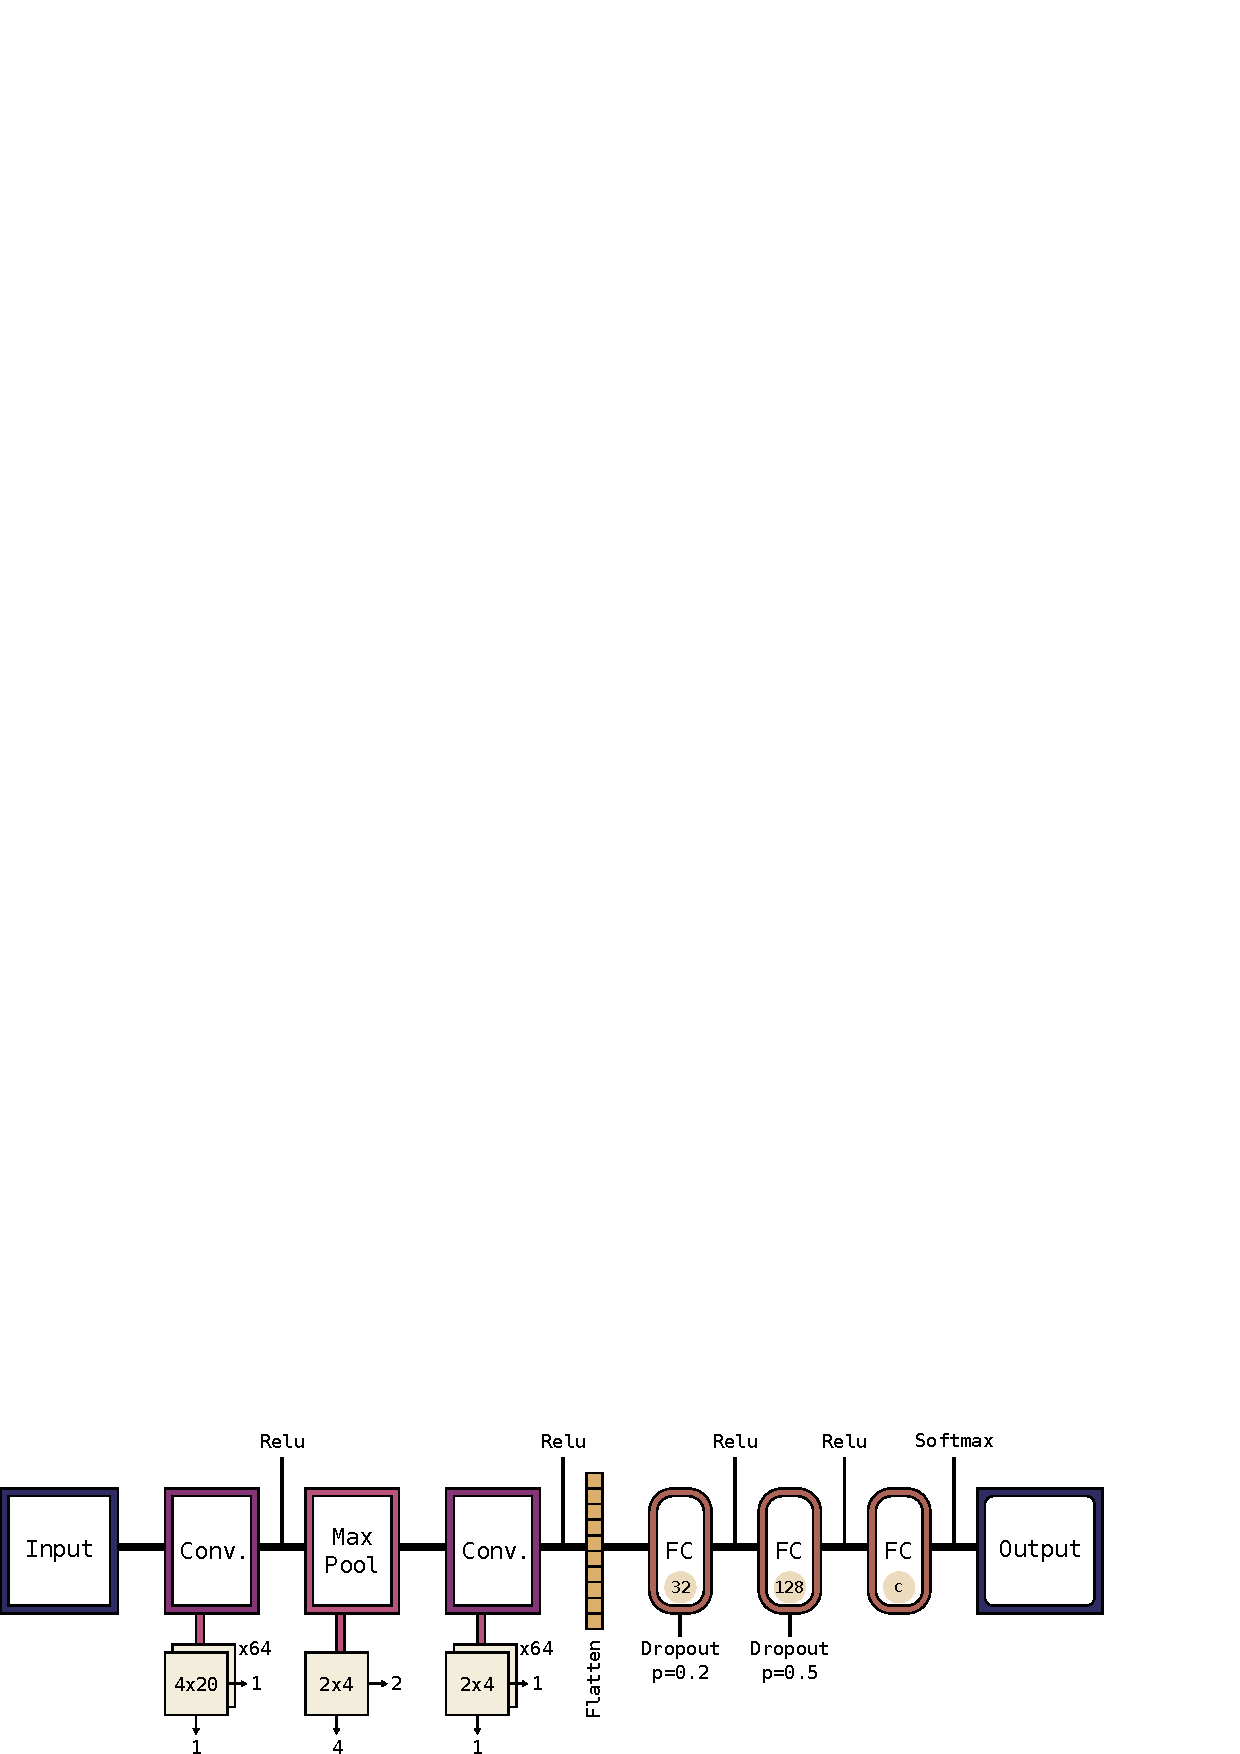
\includegraphics[height=0.35\textheight]{../4_nn/figs/nn_arch_cnn_trad.pdf} \end{figure}
\end{frame}

\begin{frame}
  \frametitle{Frequency Striding Network (conv-fstride)}
  \vspace{-0.5cm}
  \begin{itemize}
    \small
    \item Layer Structure: Conv.: 1, FC: 4
    \item Num. Params:
    \item Num. Operations: 
  \end{itemize}
  \begin{figure} 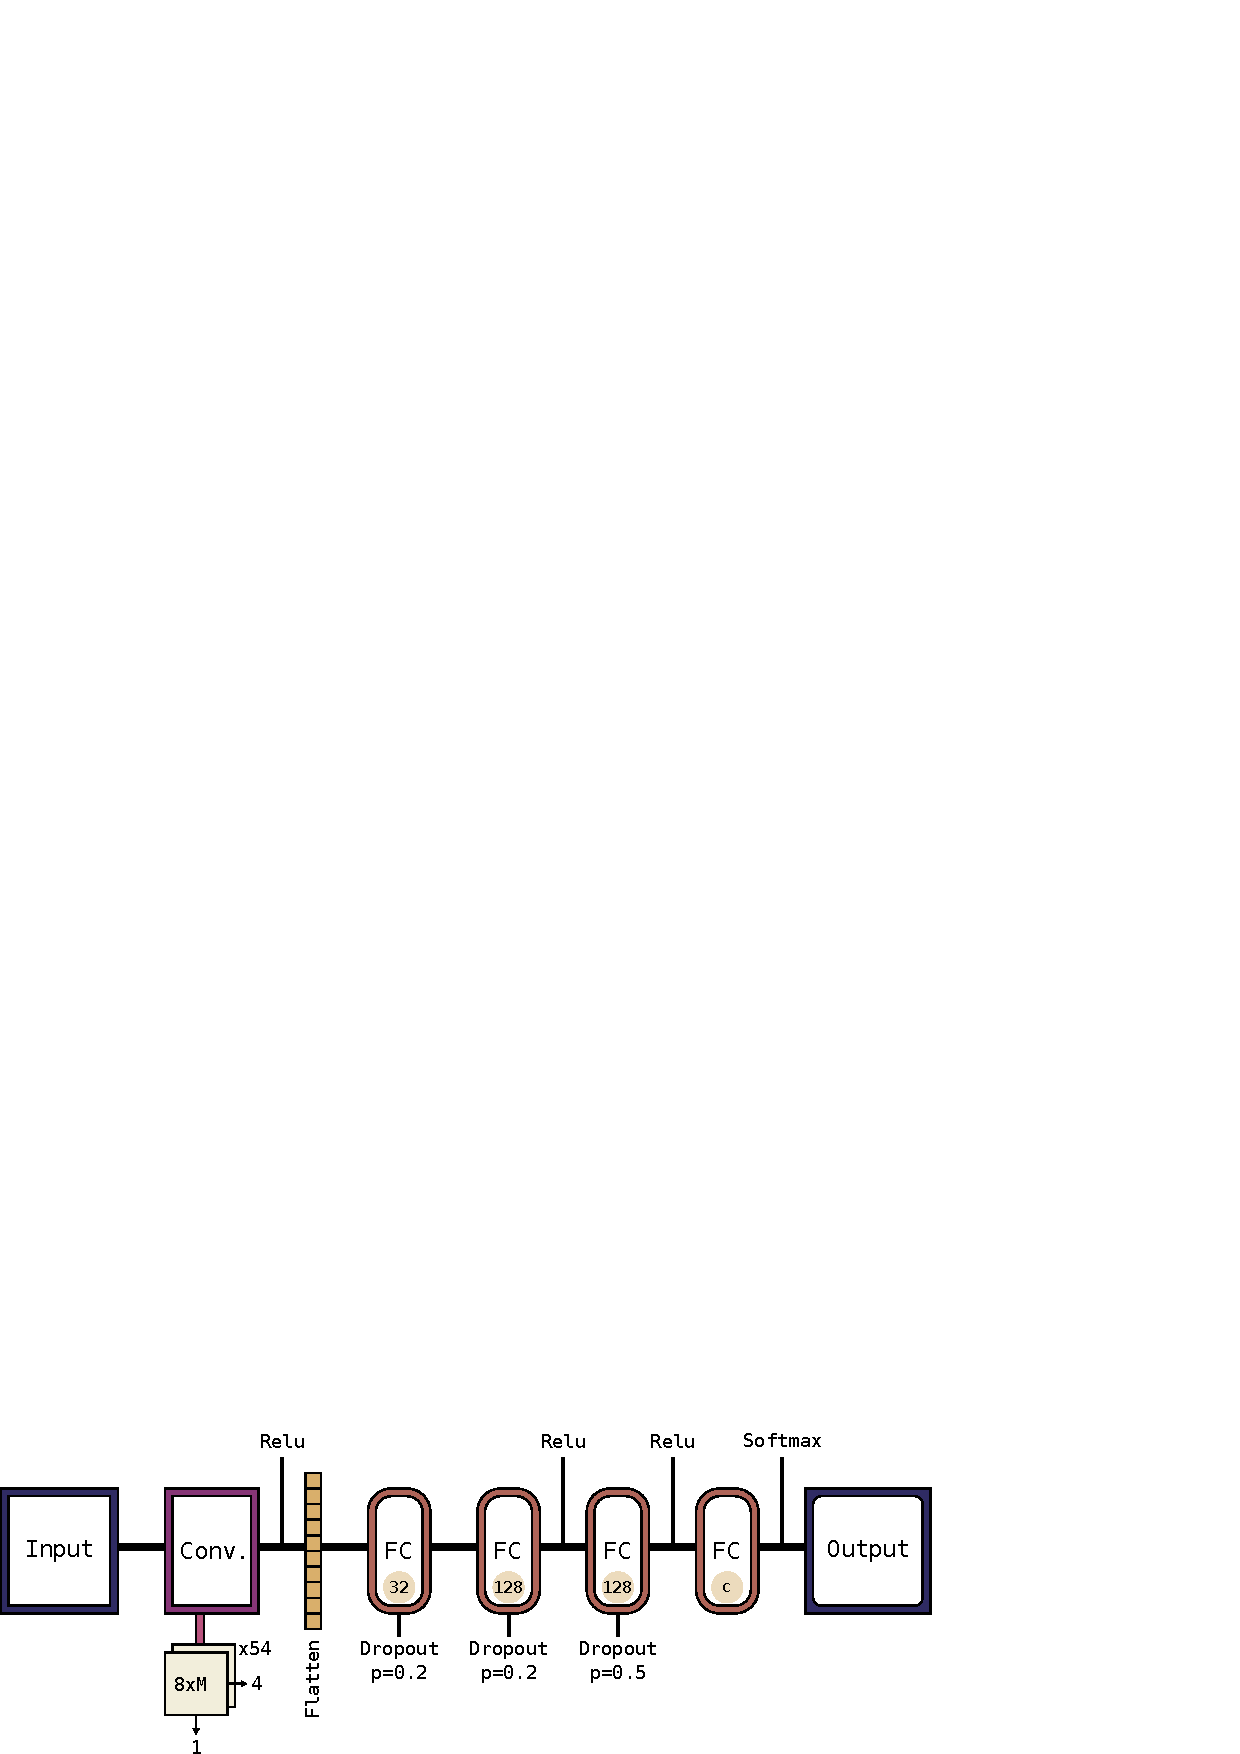
\includegraphics[height=0.35\textheight]{../4_nn/figs/nn_arch_cnn_fstride.pdf} \end{figure}
\end{frame}

\begin{frame}
  \frametitle{Time Striding Network(conv-jim)}
  \vspace{-0.5cm}
  \begin{itemize}
    \small
    \item Layer Structure: Conv.: 2, FC: 3
    \item Num. Params:
    \item Num. Operations: 
  \end{itemize}
  \begin{figure} \includegraphics[height=0.35\textheight]{../4_nn/figs/nn_arch_cnn_jim.pdf} \end{figure}
\end{frame}

